\documentclass[a4paper, times, 10pt,twocolumn]{article}
\usepackage[top=4.9cm,bottom=3.7cm,left=1.5cm,right=1.5cm]{geometry}
\usepackage{ICMLC}
\usepackage{times}
\usepackage{graphicx}
\usepackage{indentfirst}
\usepackage{latexsym}
%option
%\newtheorem{definition}{Definition}
%\newtheorem{example}{Example}
%\renewcommand{\tablename}{TABLE}
%\renewcommand{\figurename}{FIGURE}
\usepackage[margin=8pt,font=footnotesize,labelfont=bf,labelsep=period
]{caption}

%balance package is an option
%\usepackage{balance}
%\balance
%-------------------------------------------------------------------------

\pdfpagewidth=\paperwidth
\pdfpageheight=\paperheight
\pagestyle{empty}

%-------------------------------------------------------------------------
\begin{document}

\title{A Multi-stage Cascaded Encoder-decoder Framework for CT-to-PET Image Conversion in Lung Imaging}  % The title should be in Upper case

\author{\bf{\normalsize{Xiaoyu Deng${^1}$, Kouki Nagamune${^2}$, Hiroki Takada${^1}$}}\\ % The author should be in Upper case
\\
\normalsize{$^1$University of Fukui, 3-9-1 Bunkyo, Fukui, 910-0019, Japan}\\
\normalsize{$^2$University of Hyogo, 2167 Shosha, Himeji, Hyogo, 670-2280, Japan} \\
\normalsize{E-MAIL: takada@g.u-fukui.ac.jp}\\
\\}


\maketitle \thispagestyle{empty}

\begin{abstract}
   {The abstract using Times New Roman font with point size 9. The abstract is an essential part of the paper. Use short, direct, and complete sentences. It shoulds be as brief as possible and concise. It should be complete, self-explanatory, and not require reference to the paper itself. The abstract should be informative giving the scope and emphasize the main conclusions, results, or significance of the work described. Do not use the first person; do not include mathematical expressions; do not refer to the reference, and try to avoid acronyms.}
\end{abstract}
%-------------------------------------------------------------------------
\begin{keywords}
   {Tracking; Estimation; Information fusion; Resource
    management; Using point size 9}
\end{keywords}

%-------------------------------------------------------------------------
\Section{Introduction}

These are instructions for authors typesetting for {\it the International Conference on Machine Learning and Cybernetics (ICMLC) and the International Conference on Wavelet Analysis and Pattern Recognition (ICWAPR).} This document has been prepared using the required format. The electronic copy of this document can be found in: http://www.icmlc.com/.

The paper is to be written in two-column format and be right and left justified. The column width should be 8.5 cm (3.35 inches). The gap between the two columns should be 0.5 cm (0.2 inches)




%-------------------------------------------------------------------------
\SubSection{Instructions for authors}

In order for the proceedings to be ready for distribution at the conference, an electronic copy of the final version of your paper (the Camera-Ready paper) must be submitted (WORD and PDF format) to the web site. Please follow the submission instructions shown on the web site.

%-------------------------------------------------------------------------
\Section{Formatting instructions}

MS Word users: please use the paragraph styles contained in this document: Title, Author, Affiliation, Abstract, Keywords, Body Text, Equation, Reference, Figure, and Caption. Try not to change the styles manually. The size of top, bottom, left and right margins are: 4.9 cm (1.93 inches), 3.7 cm (1.46 inches), 1.5 cm (0.59 inches) and 1.5 cm (0.59 inches).

%-------------------------------------------------------------------------
\SubSection{Length}

Papers should be limited to 6 pages. Papers longer than 6 pages will be subject to extra fees based on their length.

%-------------------------------------------------------------------------
\SubSection{Title}

Type the title approximately 4.9 centimeters (1.93 inches) below the top border of the A4 paper sheet and use Times New Roman font with 14 point size in capital letters. Center the title (horizontally) on the page. Leave approximately 0.6 cm (0.24 inches) between the title and the name (in capital letters) and affiliation of yourself (and of your co-authors, if any), 0.6 cm (0.24 inches) between the name and affiliation, 1.8 cm (0.72 inches) between the affiliation and abstract. Type name(s), affiliation (s) and email(s) in 10 points and center them (horizontally) on the page.

%------------------------------------------------------------------------
\SubSection{Spacing}

Each section (or subsection) should be separated from the previous text by 0.6 cm (0.24 inches) (as indicated in the format/paragraph menu).

%-------------------------------------------------------------------------
\SubSection{Section and subsection headings}

Number section and subsection headings consecutively in Arabic numbers and type them in bold. Use point size 10 for section headings and 10 for subsection headings. Avoid using too many capital letters. Keep section and subsection headings always flushed left. If any further subdivision of a subsection is needed the titles should be 10 point.

%-------------------------------------------------------------------------
\SubSection{Main text}

Use 1.5 centimeters (0.6 inches) for the left and right margins. Use Times New Roman and font size 10 for text (character size). Do not use bold font in the main text; if you want to emphasize specific parts of the main text, use italics. Start a new paragraph by indenting it from the left margin (and not by inserting a blank line), except under a section or subsection heading. The text should be prepared with a double column format and single line spacing.

%-------------------------------------------------------------------------
\SubSection{Tables}

All tables must be numbered consecutively (in Arabic numbers). Table headings should be placed (centered) above the table. Place tables as close as possible to where they are mentioned in the main text. 
% \begin{table}[h]
% \footnotesize
% \centering
% \caption{Table type styles}
% %\begin{tabular}{cccc}
% \begin{tabular}{p{1cm}p{3cm}p{1.5cm}p{1.5cm}}
% \hline
% Table &\multicolumn{3}{c}{Table Column Head}\\ \cline{2-4}
% head & \emph{Table column subhead} & \emph{subhead} & \emph{subhead}\\ \hline
% row 1 & aaa & aaa & aaa \\
% row 2 & bbb & bbb & bbb \\
% \hline
% \end{tabular}
% \end{table}
\begin{table}[h]
	% \centering
	\caption{Encoder-decoder Setting Table}
	\label{tab:encoder_setting}
	\begin{tabular}{ccccc}
		\hline
		Block Name   & input & output & trans & dropout \\
		\hline
		Encoder 1    & 3     & 16     & -     & -       \\
		Encoder 2    & 16    & 24     & -     & -       \\
		Encoder 3    & 24    & 42     & -     & -       \\
		Encoder 4    & 42    & 81     & -     & -       \\
		Encoder 5    & 81    & 114    & -     & -       \\
		Encoder 6    & 114   & 162    & -     & -       \\
		Encoder 7    & 162   & 162    & -     & -       \\
		Encoder 8    & 162   & 960    & -     & -       \\
		Decoder 1    & 960   & 960    & 162   & 0.5     \\
		Decoder 2    & 1122  & 162    & 162   & 0.5     \\
		Decoder 3    & 324   & 114    & 114   & 0.5     \\
		Decoder 4    & 228   & 81     & 81    & -       \\
		Decoder 5    & 162   & 42     & 42    & -       \\
		Decoder 6    & 84    & 24     & 24    & -       \\
		Decoder 7    & 48    & 16     & 16    & -       \\
		Visual Block & 32    & 3      & -     & -       \\
		\hline
	\end{tabular}
\end{table}


\begin{table}[h]
	\centering
	\caption{Parameters of Neural Networks.}
	\label{tab:model_parameters}
	\begin{tabular}{ccccc}
		\hline
		Architectures                                                   & Parameters \\
		\hline
		U-Net\cite{navab_u-net_2015}                                    & 54.41      \\
		Cas-UNet\cite{zeng_swin-casunet_2022}                           & 108.82     \\
		DualStageGGAN\cite{wang_dsg-gandual-stage-generator-based_2024} & 92.54      \\
		Stage01                                                         & 22.13      \\
		Stage02                                                         & 44.26      \\
		Stage03                                                         & 66.39      \\
		Stage04                                                         & 88.52      \\
		Stage05                                                         & 110.65     \\
		Stage06                                                         & 132.77     \\
		Stage07                                                         & 154.90     \\
		Stage08                                                         & 177.03     \\
		Stage09                                                         & 199.16     \\
		Stage10                                                         & 221.29     \\
		\hline
		\multicolumn{2}{p{201pt}}{The table depicts the Parameters of different generators. The quantity of parameters is expressed in millions.}
	\end{tabular}
\end{table}

%-------------------------------------------------------------------------
\SubSection{Figures}

All illustrations should be original drawings or photographic prints
of originals. Photographs should be glossy prints. Photocopies are
often not good enough and should be avoided. All illustrations must
be numbered consecutively (i.e., not section-wise), using Arabic
numbers.  Center figure captions beneath the figure (see Figure 1).
If possible, do not assemble figures at the back of your article,
but place them as close as possible to where they are mentioned in
the main text. No part of a figure should go beyond the typing area.
Captions should appear (centered) below graphical objects, as in
Figure \ref{Fig:Figure 1}.
%------------------------figure---------------------------------------
\begin{figure*}[t!]
	\centering
	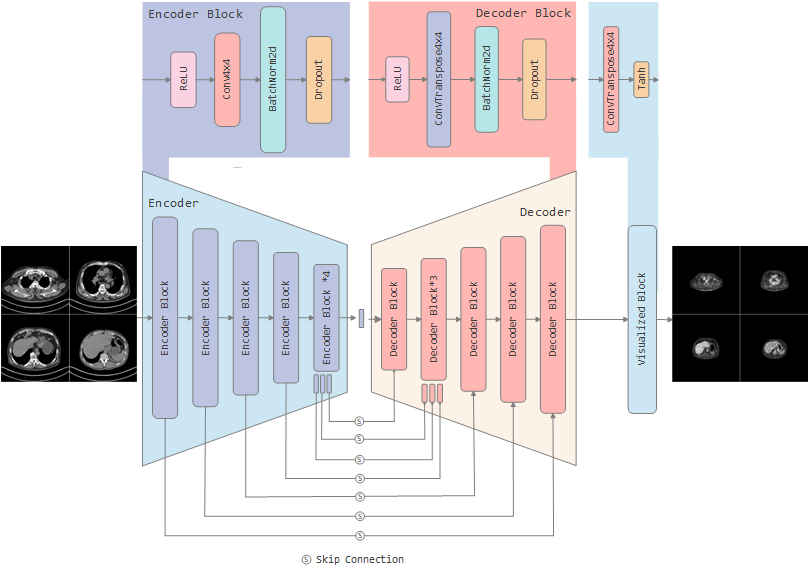
\includegraphics[width=1.0\linewidth]{u-net/lung/Encoder-Decoder-5layer-250406}
	\caption[architecture]{Schematic Diagram of Data Flow Within the Model. The PET image is shown on the left, and the CT image on the right. The blue modules correspond to the encoder architecture, while the orange modules represent the decoder architecture. The upper portion of the figure illustrates the fundamental structures of the encoder blocks, decoder blocks, and visualization blocks. The connections in the lower portion indicate the skip connections.}
	\label{fig:Encoder_Decoder_Pair}
\end{figure*}

%-------------------------------------------------------------------------
\SubSection{Mathematical formulas}

Mathematical formulas should be roughly centered and have to be
numbered as formula (\ref{Eq-1}).
%--------------------------------------------------
\begin{equation}\label{Eq-1}
\centering{y=f(x)}
\end{equation}

%-------------------------------------------------------------------------
\SubSection{References}

References to the literature should be mentioned in the main text by
an Arabic number in square brackets \cite{Peter}, \cite{John}. List
these (in cited order) at the very end of your paper (under the
heading References). Start each reference on a new line with its
number in square brackets \cite{Xizhao}.

%-------------------------------------------------------------------------
\SubSection{Copyright form and copyright notice}

One of the authors must submit a signed copyright form to the
Publications Chair before the final version of the paper can be
accepted for publication. The copyright form is available from the
conference web site.
%-------------------------------------------------------------------------
\SubSection{Fine tuning}

\hspace{-3ex}    $\bullet$ \hspace{1ex} Do not end a page with a
section or subsection heading.

 \hspace{-3ex}    $\bullet$ \hspace{1ex} Do not include page numbers in the text.


%-------------------------------------------------------------------------
\SubSection{Final version}

After proofreading your paper, it must be submitted on the ICMLC or ICWAPR web site electronically using WORD and PDF format.
{\it Do not send hard copies or use other file formats - they will
not be accepted.} Proper usage of the English language is expected
of all submissions (i.e., Camera-ready papers). Make sure that the
PDF file looks fine on the screen as well as in print.

In order to build the indices for the CD-ROM, we need the title and
author information for your paper entered into the PDF file.

In Acrobat, select the menu option File $\longrightarrow$ Document
Properties $\longrightarrow$ Summary and then fill in your paper
title and author information.

In Word, select the menu option File $\longrightarrow$ Properties,
and then fill in the dialog box with your paper's title and author
information.

Please use only the standard fonts that come with the system and
standard font encoding schemes. If you use your own fonts, please
make sure that the fonts are fully embedded into the PDF file. If
you create your file on an operating system running a language other
than English, please make sure that your file can be opened
correctly on all computers. Missing fonts and different font
encoding schemes are the main reasons for read errors in Acrobat.

Failure to follow the above guidelines may result in a submission
being rejected for publication in the conference proceedings and CD
ROM.

\newpage
%------------------------------------------------------------------------
\Section{Conclusions}

In this sample paper, we have presented the formatting instructions
for ICMLC and ICWAPR.



%-------------------------------------------------------------------------
\section*{Acknowledgements}

This paper is supported by the Machine Learning Centre of the Hebei
University, Shanghai Jiaotong University, and the IEEE Systems, Man
and Cybernetics Society.

%-------------------------------------------------------------------------
%\nocite{ex1,ex2}
%\bibliographystyle{latex8}
%\bibliography{latex8}

\begin{thebibliography}{99}
%\addtolength{\itemsep}{-0.8em}
\bibitem{Peter}
Peter. C. Author, ``Paper's name'', Proceeding of ICMLC2002
Conference, Beijing, pp. 111-116, November 2002.

\bibitem{John} John. B. Author, and A. Friend, ``Journal paper's name'', Journal's
name, Vol 39, No. 1, pp. 222-226, Feb. 2001.
\bibitem{Xizhao} Xizhao Wang, His book's name, Publisher, Location, Year.
\end{thebibliography}




\end{document}
